
\section{Objetivo de cada shader e fluxo entre eles}

A técnica usa dois shaders. Eles começaram como pseudocódigo em sintaxe GLSL (arquivos originais em \texttt{pseudocodigo/}) e evoluíram para os shaders compiláveis da implementação (\texttt{código/shaders/uv\_mapping.vert} e \texttt{uv\_mapping.frag}), que são apresentados aqui como a versão final.

\begin{itemize}
    \item \textbf{Vertex shader} (\texttt{uv\_mapping.vert}): transforma a posição de cada vértice para o espaço de recorte e repassa o UV e a normal. Não altera o UV.
    \item \textbf{Fragment shader} (\texttt{uv\_mapping.frag}): recebe o UV já interpolado e, conforme o modo, lê a textura com o UV original ou deslocado, calcula o padrão procedural, mistura os dois ou desenha a grade de depuração. No fim, aplica a iluminação.
\end{itemize}

O fluxo é: atributos do vértice \(\rightarrow\) vertex shader \(\rightarrow\) rasterização, que interpola \texttt{fragUV} e \texttt{fragNormal} com correção de perspectiva (Equação~\eqref{eq:perspectiva}) \(\rightarrow\) fragment shader \(\rightarrow\) cor no color attachment. Os dois shaders compartilham o mesmo bloco \texttt{uniform} (binding~0).

\section{Entradas, saídas e recursos}

\begin{table}[H]
\centering
\caption{Entradas, saídas e recursos dos shaders.}
\label{tab:shader-io}
\small
\begin{tabular}{p{3.0cm}p{2.0cm}p{2.4cm}p{6.4cm}}
\toprule
\textbf{Nome} & \textbf{Tipo} & \textbf{Origem} & \textbf{Significado} \\
\midrule
\texttt{inPosition} & \texttt{vec3} & location 0 & Posição do vértice no espaço do modelo \\
\texttt{inNormal} & \texttt{vec3} & location 1 & Normal do vértice \\
\texttt{inUV} & \texttt{vec2} & location 2 & Coordenada de textura do glTF (\texttt{TEXCOORD\_0}) \\
\texttt{params.model}, \texttt{view}, \texttt{projection} & \texttt{mat4} & binding 0 & Matrizes de modelo (rotação), câmera e projeção \\
\texttt{params.time} & \texttt{float} & binding 0 & Segundos desde o início, \(t\) nas equações \\
\texttt{params.mode} & \texttt{int} & binding 0 & Modo de renderização, de 1 a 5 \\
\texttt{baseTexture} & \texttt{sampler2D} & binding 1 & Textura do modelo com o sampler (\texttt{LINEAR}, \texttt{REPEAT}) \\
\texttt{fragUV}, \texttt{fragNormal} & \texttt{vec2}, \texttt{vec3} & vertex \(\rightarrow\) fragment & UV e normal, interpolados por fragmento \\
\texttt{gl\_Position} & \texttt{vec4} & saída do vertex & Posição em espaço de recorte \\
\texttt{outColor} & \texttt{vec4} & saída do fragment & Cor final do pixel (location 0) \\
\bottomrule
\end{tabular}
\end{table}

\section{Vertex shader}

\begin{small}
\begin{verbatim}
#version 450
layout(set = 0, binding = 0) uniform Parameters {
    mat4 model; mat4 view; mat4 projection;  // matrizes (Eq. 3.2)
    float time; int mode;                    // tempo e modo (1 a 5)
} params;

layout(location = 0) in vec3 inPosition;     // atributos do glTF
layout(location = 1) in vec3 inNormal;
layout(location = 2) in vec2 inUV;
layout(location = 0) out vec2 fragUV;        // vao para o rasterizador
layout(location = 1) out vec3 fragNormal;

void main() {
    // posicao em espaco de recorte: P * V * M * p
    gl_Position = params.projection * params.view * params.model
                * vec4(inPosition, 1.0);
    // o UV do arquivo e repassado sem alteracao; o rasterizador
    // o interpola com correcao de perspectiva
    fragUV = inUV;
    // a matriz model e so rotacao, entao serve tambem para normais
    fragNormal = mat3(params.model) * inNormal;
}
\end{verbatim}
\end{small}

\section{Fragment shader}

\begin{small}
\begin{verbatim}
#version 450
layout(set = 0, binding = 0) uniform Parameters {
    mat4 model; mat4 view; mat4 projection; float time; int mode;
} params;
layout(set = 0, binding = 1) uniform sampler2D baseTexture;
layout(location = 0) in vec2 fragUV;
layout(location = 1) in vec3 fragNormal;
layout(location = 0) out vec4 outColor;

const int MODE_TEXTURE = 1, MODE_DYNAMIC_UV = 2, MODE_PROCEDURAL = 3,
          MODE_BLEND = 4,   MODE_UV_GRID = 5;

// UV DINAMICO (Eqs. 3.5 e 3.6): a malha fica parada, o UV se move
vec2 dynamicUV(vec2 uv, float t) {
    uv.x += t * 0.10;                              // translacao
    uv.x += sin(uv.y * 12.0 + t * 2.0) * 0.015;    // ondulacao em u
    uv.y += cos(uv.x * 12.0 + t * 1.5) * 0.015;    // ondulacao em v
    return uv;   // pode sair de [0,1]: o sampler REPEAT da a volta
}

// PADRAO PROCEDURAL (Eq. 3.11): cor gerada por funcoes, sem imagem.
// Retorna a cor em rgb e a "energia" da onda em a.
vec4 proceduralPattern(vec2 uv, float t) {
    uv.x += t * 0.40;                              // deslocamento
    uv.y += sin(t * 1.2) * 0.10;
    float dx = sin(uv.y * 14.0 + t * 2.0) * 0.08;  // distorcao: as duas
    float dy = cos(uv.x * 12.0 - t * 1.5) * 0.08;  // partes usam o uv
    uv += vec2(dx, dy);                            // anterior a ela
    float w1 = sin(uv.x * 20.0 + uv.y * 8.0 + t * 4.0);   // 3 ondas
    float w2 = sin(uv.y * 24.0 - uv.x * 6.0 - t * 3.0);
    float w3 = sin((uv.x + uv.y) * 18.0 + t * 2.0);
    float e = ((w1 + w2 + w3) / 3.0) * 0.5 + 0.5;  // normaliza p/ [0,1]
    vec2 g = fract(uv * 8.0);                      // grade 8x8 (Eq. 3.8)
    float grid = max(smoothstep(0.46, 0.50, abs(g.x - 0.5)),
                     smoothstep(0.46, 0.50, abs(g.y - 0.5)));
    vec3 c = mix(vec3(0.005, 0.015, 0.12), vec3(0.0, 0.18, 0.85), e);
    c = mix(c, vec3(0.0, 0.85, 1.0), smoothstep(0.55, 0.90, e));
    c = mix(c, vec3(0.65, 1.0, 1.0), smoothstep(0.90, 1.0, e));
    c = mix(c, c * 0.35, grid * 0.25);             // escurece a grade
    c += vec3(0.0, 0.25, 0.35) * pow(e, 3.0);      // brilho
    return vec4(c, e);
}

// GRADE UV (depuracao): U em vermelho, V em verde, xadrez 10x10
vec3 uvGrid(vec2 uv) {
    vec2 cells = uv * 10.0;
    float checker = mod(floor(cells.x) + floor(cells.y), 2.0);
    vec2 d = abs(fract(cells) - 0.5);
    float line = smoothstep(0.44, 0.48, max(d.x, d.y));
    vec3 c = vec3(fract(uv.x), fract(uv.y), 0.2) * (0.65 + 0.35 * checker);
    return mix(c, vec3(1.0), line);
}

void main() {
    float t = params.time;
    // iluminacao difusa (Eq. 3.14); a normal interpolada e renormalizada
    vec3 n = normalize(fragNormal);
    float diffuse = max(dot(n, normalize(vec3(0.4, 0.8, 0.6))), 0.0);
    float lighting = 0.35 + 0.65 * diffuse;
    vec3 color;
    if (params.mode == MODE_TEXTURE)
        color = texture(baseTexture, fragUV).rgb * lighting;
    else if (params.mode == MODE_DYNAMIC_UV)
        color = texture(baseTexture, dynamicUV(fragUV, t)).rgb * lighting;
    else if (params.mode == MODE_PROCEDURAL)
        color = proceduralPattern(fragUV, t).rgb * (0.55 + 0.45 * diffuse);
    else if (params.mode == MODE_UV_GRID)
        color = uvGrid(fragUV) * lighting;
    else {  // MODE_BLEND (e qualquer valor fora de 1..5)
        vec3 tex = texture(baseTexture, dynamicUV(fragUV, t)).rgb * lighting;
        vec4 p = proceduralPattern(fragUV, t);
        color = mix(tex, p.rgb, smoothstep(0.45, 0.95, p.a) * 0.75);
    }
    outColor = vec4(color, 1.0);
}
\end{verbatim}
\end{small}

\section{Equações e variáveis}

Cada cálculo do shader corresponde a uma equação do Capítulo~\ref{chap:equacoes}, onde estão o significado de cada variável e o estágio em que ela é executada: posição (Eq.~\ref{eq:mvp}), translação (Eq.~\ref{eq:translacao}), ondulação (Eq.~\ref{eq:onda}), repetição (Eq.~\ref{eq:repeat}), escala (Eq.~\ref{eq:escala}), padrão procedural e misturas (Eqs.~\ref{eq:procedural} e~\ref{eq:mix}) e iluminação (Eq.~\ref{eq:lambert}). As funções GLSL usadas são \texttt{mix(a,b,x)} \(= a(1-x)+bx\); \texttt{smoothstep(e0,e1,x)}, uma transição suave de 0 a 1 entre \(e_0\) e \(e_1\); \texttt{fract(x)} \(= x-\lfloor x\rfloor\); e \texttt{normalize}, que divide o vetor pela sua norma.

\section{Condições e laços}

O fragment shader tem uma única cadeia de condições, sobre \texttt{params.mode}, que escolhe um de cinco cálculos. Como \texttt{mode} vem do Uniform Buffer, o valor é o mesmo para todos os fragmentos do quadro: todas as threads seguem o mesmo ramo e não há divergência. Não há laços: as três ondas do padrão procedural são uma soma de tamanho fixo, escrita explicitamente, e nenhum cálculo depende de vizinhos ou de iterações. O critério de parada, portanto, não se aplica. Cada fragmento executa um número constante de operações (Tabela~\ref{tab:custo-modos}).

\section{Amostragem da textura}

A textura é lida com \texttt{texture(baseTexture, uv)} nos modos 1, 2 e 4. O sampler é configurado na aplicação (Capítulo~\ref{chap:vulkan}) com:
\begin{itemize}
    \item filtragem \texttt{LINEAR} na ampliação e na redução, que interpola os quatro texels mais próximos;
    \item endereçamento \texttt{REPEAT}, que aplica a Equação~\eqref{eq:repeat} ao UV deslocado;
    \item anisotropia no máximo suportado pela GPU;
    \item modo de mipmap \texttt{LINEAR}.
\end{itemize}
Como a imagem tem um único nível, o nível de detalhe calculado pela GPU (Equação~\eqref{eq:lod}) não tem efeito. Essa limitação está registrada na Tabela~\ref{tab:otimizacoes}. O padrão procedural e a grade não leem textura: são calculados diretamente a partir do UV.

\section{Tratamento de limites e valores inválidos}

\begin{itemize}
    \item \textbf{UV fora de \([0,1]\):} o deslocamento faz \(u\) crescer sem limite. Quem trata isso é o sampler (\texttt{REPEAT}), e não o shader. A grade usa \texttt{fract} pelo mesmo motivo.
    \item \textbf{Normal interpolada:} não é unitária, por isso é renormalizada. Uma normal nula produziria NaN, mas o modelo glTF sempre fornece normais.
    \item \textbf{Luz por trás da superfície:} \texttt{max(dot, 0)} impede iluminação negativa, e o termo constante de 0,35 evita regiões totalmente pretas.
    \item \textbf{Energia procedural:} a soma das ondas, no intervalo \([-3,3]\), é normalizada para \([0,1]\) antes de servir de peso nas misturas, o que garante que \texttt{mix} e \texttt{smoothstep} recebam valores válidos.
    \item \textbf{Cor acima de 1:} o brilho do padrão procedural pode somar até \(0{,}35\) ao canal azul e levar a cor acima de 1. O shader não aplica \texttt{clamp}: como o color attachment usa um formato normalizado de 8 bits, a GPU limita cada canal a \([0,1]\) na escrita.
    \item \textbf{Modo inválido:} qualquer valor fora de 1 a 5 cai no último ramo (mistura). Na aplicação, o valor só muda pelas teclas 1 a 5.
\end{itemize}

\section{Resultado esperado e relação com a técnica}

O vertex shader produz a posição do vértice na tela, e o fragment shader produz a cor de cada pixel do modelo. A Figura~\ref{fig:app-modos} mostra os modos 1, 3, 4 e 5; o modo~2 está na Figura~\ref{fig:app-uv-dinamico}.

\begin{figure}[H]
    \centering
    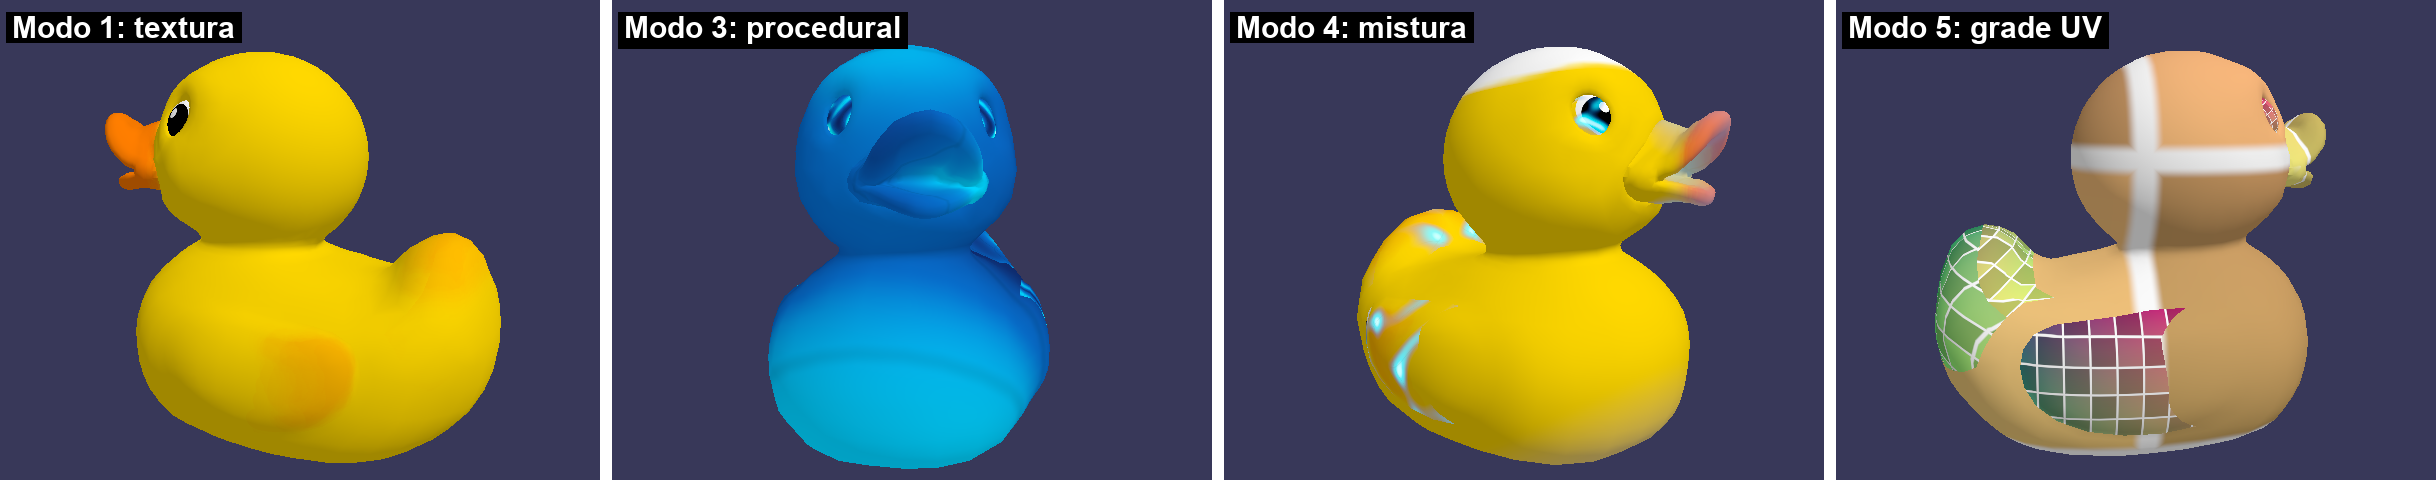
\includegraphics[width=\textwidth]{imagens/marcadas/app_modos.png}
    \caption{Resultado dos shaders na implementação (capturas próprias, \texttt{código/evidencias/}).}
    \label{fig:app-modos}
\end{figure}

Resultado esperado de cada modo:
\begin{enumerate}
    \item a textura original do modelo;
    \item a mesma textura deslizando e ondulando sobre a malha parada (Figura~\ref{fig:app-uv-dinamico});
    \item ondas azuis e ciano geradas sem imagem;
    \item a textura deslizando com ondas de luz por cima;
    \item a grade de depuração, que revela o esticamento e as costuras do UV.
\end{enumerate}
O modo~2 implementa o UV mapping dinâmico (a parametrização muda a cada quadro), o modo~3 o mapeamento procedural (a cor vem de uma função) e o modo~4 a combinação dos dois.
